\documentclass{article}
\usepackage[a4paper, paperwidth=25cm, paperheight=25.5cm, left=1.5cm, right=1.5cm, top=1cm, bottom=2cm]{geometry}
\usepackage{tikz,tcolorbox}
\usepackage{amsmath}
\usepackage[table,xcdraw]{xcolor}
\usepackage{listings}
\usepackage{array,multirow} % For customizing tables
\usepackage{booktabs} % For better horizontal lines
\usepackage{makecell}
\setlength{\parindent}{0pt}

\tcbuselibrary{skins, breakable, theorems}

\definecolor{myblue}{HTML}{10C2C4}

\newtcolorbox{prettyBox}[2]{
  enhanced,
  colback=white!90!#2,   % Background color based on the second parameter (color)
  colframe=#2!60!black,  % Frame color based on the second parameter (color)
  coltitle=white,        % Title color (white)
  fonttitle=\bfseries\Large,
  title=#1,              % Title from the first parameter
  boxrule=1mm,
  arc=0.5mm,
  drop shadow=#2!35!gray, % Drop shadow color based on the second parameter (color)
}

\usepackage{listings}
% Define the style for C code
\lstdefinestyle{cstyle}{
    language=C,
    basicstyle=\ttfamily\small,
    keywordstyle=\color{blue}\bfseries,
    stringstyle=\color{red},
    commentstyle=\color{green!50!black}\itshape,
    numbers=left,
    numberstyle=\tiny\color{gray},
    stepnumber=1,
    breaklines=true,
    frame=tb,
    tabsize=4,
    showstringspaces=false,
    captionpos=b
}


\lstdefinestyle{pythonstyle2}{
    language=python,                    % Language set to Python
    basicstyle=\ttfamily\footnotesize,   % Change basic font size
    keywordstyle=\color{blue}\bfseries, % Different keyword style
    stringstyle=\color{red},         % Different string color
    commentstyle=\color{green!60!black}\itshape, % Adjust comment color
    numbers=left,                       % Line numbers on the left
    numberstyle=\tiny\color{gray},      % Smaller number font and color
    stepnumber=1,                       % Number each line
    frame=single,                       % Single frame around code
    tabsize=4,                          % Adjust tab size
    showstringspaces=false,             % Do not show spaces in strings
    captionpos=b,% Position of caption
    breaklines=true,
    inputencoding=utf8
}




\begin{document}
\begin{center}
    \Huge{\textbf{\underline{Chapter 1: Introduction}}}
\end{center}

\vspace{0.35cm}


\section{Numerical Algorithm (Numerical Method)}
\begin{prettyBox}{Numerical Algorithm}{mygreen}
A Numerical Algorithm provides an approximate solution and is used to solve problems involving large amounts of data. The algorithm is based on a well-defined iterative sequence, starting with an initial solution that progressively converges toward the desired result with each iteration.

\[
\begin{cases}
    \hspace{0.1cm}(U_n) & \hspace{-0.1cm}n \geq 0 \\[0.15cm]
    \hspace{0.1cm}S_0 & \hspace{-0.3cm} \text{Initial Solution (Starting Point)}
\end{cases}
\]
\end{prettyBox}
\vspace{0.35cm}

\section{Convergence Speed (Order of Convergence)}
\begin{prettyBox}{Convergence Speed}{mygreen}
The number of iterations required to find the solution we are looking for:
\begin{itemize}
    \item Linear Order: 1 (slow)
    \item Quadratic Order: 2 (faster)
    \item \(>>\) 2 (very fast)
\end{itemize}
\end{prettyBox}

\vspace{0.35cm}

\section{Interpolation}
\begin{prettyBox}{Interpolation}{mygreen}
Estimates the value between two known points of a function allowing for a smoother representation of the function's behavior.
\end{prettyBox}

\vspace{0.35cm}

\section{Approximation}
\begin{prettyBox}{Approximation}{mygreen}
Approximates the formula of a function from a set of values, with the objective of finding a simpler function that represents the general trend of the data, even if it doesn't pass through every point exactly.
\end{prettyBox}

\vspace{0.35cm}

\section{Error}
\begin{prettyBox}{Error}{mygreen}
An error represents the difference between the actual solution and the computed result. It indicates how far we are from the true solution. There are two cases:
\begin{itemize}
    \item \textbf{Evaluation}: We know the exact solution, so we can directly calculate the error:
        \[   \boxed{E_r = |\overline{x} - x_{\text{app}}|} \]
    \item \textbf{Estimation}: We don't know the exact solution, so we only have an estimate of the error, based on the output of the algorithm:
        \[      \boxed{E_r = |\overline{x} - x_{\text{app}}| \leq \text{Algo}} \]
\end{itemize}

Where:
\begin{itemize}
    \item \(E_r\) : The error value.
    \item \(\overline{x}\) : The exact solution.
    \item \(x_{\text{app}}\) : The approximate solution.
    \item Algo : The error value found by the algorithm.
\end{itemize}
\end{prettyBox}

\vspace{0.35cm}

\section{Optimization}
\begin{prettyBox}{Optimization}{mygreen}
Optimization in numerical algorithms refers to two things:
\begin{itemize}
    \item \textbf{Error}: We aim to minimize the error in order to achieve the most accurate approximate solution.
    \item \textbf{Convergence Speed}: The higher the order of convergence, the less time the algorithm will take to converge to the solution we are looking for.
\end{itemize}
\end{prettyBox}

 
\section{File Management}

\subsection{What's A File Management}

\subsection{Objective Of A File Management}

\subsection{Concept Of File}

\subsection{Concept Of Repository}

\subsection{UNIX Solution}
 
\newpage
\null
\vspace{0.15cm}

\begin{center}
    \Huge{\textbf{\underline{Chapter 3: Communication Between Processes}}}
\end{center}

\setcounter{section}{0}

\vspace{0.35cm}


\section{Introduction}

\begin{prettyBox}{Introduction}{myblue}
When processes communicate with each other, it is called \textbf{Inter-Process Communication (IPC)}. IPC allows processes to share information and work together. There are two main scenarios: 
\begin{itemize}
    \item \textbf{Same Process}: A single program is divided into threads or split into child processes that communicate internally.
    \item \textbf{Different Processes}: Two separate programs running at the same time exchange information.
\end{itemize}
\end{prettyBox}

\vspace{0.35cm}

\section{Same Process}

\subsection{Child Processes}
\begin{prettyBox}{Child Processes}{myblue}
The parent process is the first instance of the program, which is split into child
processes using the primitive \textbf{fork()} that inherit all variables from parent and start executing after the fork. These processes communicate with
each other and with their parent through pipes.
\end{prettyBox}

\vspace{0.35cm}

\subsubsection{Fork}

\begin{prettyBox}{fork()}{myblue}
To use \textbf{fork()}, include the \texttt{<unistd.h>} header  
,the \textbf{fork()} function splits the current process into two: a parent process and a child process. It returns a process ID (\textbf{pid}) with the following results:
\begin{itemize}
    \item \textbf{fork() = -1} : Error, fork failed.
    \item \textbf{fork() = 0} : PID of the child process.
    \item \textbf{fork() \(>\) 0} : PID of the parent process.
\end{itemize}
\end{prettyBox}

\newpage
\null

\lstinputlisting[style=cstyle]{Chapters/C/Fork/ex1.c}


\vspace{0.5cm}

\begin{prettyBox}{exit()}{red}
    Terminates the current process with the given status. Use:
    \begin{itemize}
        \item \texttt{0} for a successful termination.
        \item \texttt{-1} for indicating an error.
    \end{itemize}
\end{prettyBox}

\vspace{0.35cm}

\begin{prettyBox}{When Forking Fails}{red}
    \begin{itemize}
        \item Exceeded the maximum number of child processes.
        \item Not enough memory or resources to fork.
    \end{itemize}
\end{prettyBox}

\vspace{0.35cm}

\subsubsection{Wait}
\begin{prettyBox}{wait(NULL)}{myblue}
To use \textbf{wait(NULL)}, include the \texttt{<sys/wait.h>} header used by parent processes , wait for its child processes to terminates
\end{prettyBox}

\newpage
\null
\lstinputlisting[style=cstyle]{Chapters/C/Fork/ex2.c}

\vspace{0.35cm}
\subsubsection{Pipe}
\begin{prettyBox}{pipe()}{myblue}
To use \texttt{pipe()} we need to include the header \texttt{<unistd.h>}\\
    The \texttt{pipe()} function creates a pipe and takes an array of two integers as input:
    \begin{itemize}
        \item \texttt{pipe(descriptor)} creates the pipe and stores the file descriptors in the \texttt{descriptor} array , if pipe creation fails, \texttt{-1} is returned.
    \end{itemize}
    The two elements of the \texttt{descriptor} array represent the ends of the pipe:
    \begin{itemize}
        \item \texttt{read(descriptor[0], \&var, sizeof(var))} reads from the pipe.
        \item \texttt{write(descriptor[1], \&var, sizeof(var))} writes to the pipe.
    \end{itemize}
    To close a pipe end, use the \texttt{close(descriptor[i])} function.

\end{prettyBox}


\newpage
\null

\begin{prettyBox}{Reminder}{red}
\textbf{Frequent Mistakes With Pipes}
\begin{itemize}
    \item \textbf{Closing All Read Descriptors Then Trying To Write On Pipe}: 
    Kernel doesn't find where to write the data, causing a SIGPIPE signal or an EPIPE error.
    \item \textbf{Not Closing All Write Descriptors Then Trying To Read From That Pipe}: 
    Kernel waits for the pipe to be written to, as it doesn't see an EOF (End Of File) signal.
\end{itemize}

\textbf{Solution}
\begin{itemize}
    \item \textbf{Leave at least one read end of the pipe open before writing to it}, 
    so the kernel knows where to write the data.
    \item \textbf{Always close all write ends of a pipe before reading from it}, 
    so the kernel knows that the pipe has reached its EOF.
\end{itemize}

\end{prettyBox}


\vspace{0.35cm}
\begin{prettyBox}{Note}{red}
    You can loop through \texttt{read()} using \texttt{read() > 0}, as it returns the number of bytes read. 
    As data is read, the cursor moves until \textbf{EOF} (End of File) is reached.
\end{prettyBox}

\vspace{1.25cm}

\subsubsection*{\underline{Example}}

\begin{itemize}
    \item \textbf{child\_1}: Accepts input of n characters. Write only alphabetic characters to the pipe, converts lowercase letters to uppercase. Stops when the user inputs '0'.
    \item \textbf{child\_2}: Prints the characters written to the pipe by \textbf{child\_1}.
    \item \textbf{parent}: Creates the child processes and waits for them to finish.
\end{itemize}

\newpage

\subsubsection*{\underline{Code Overview}}
\lstinputlisting[style=cstyle,basicstyle=\footnotesize\ttfamily]{Chapters/C/Fork/ex3.1.c}

\newpage

\subsubsection*{\underline{child\_1 function :}}
\lstinputlisting[style=cstyle,basicstyle=\footnotesize\ttfamily]{Chapters/C/Fork/ex3.2.c}

\vspace{0.5cm}

\subsubsection*{\underline{child\_1 function :}}
\lstinputlisting[style=cstyle,basicstyle=\footnotesize\ttfamily]{Chapters/C/Fork/ex3.3.c}

\vspace{1cm}

\begin{itemize}
    \item \textbf{parent}: Write 5 integers.
    \item \textbf{child}: Read the integers of parent and write their double.
    \item \textbf{parent}: Read Double integers of child.
\end{itemize}

\newpage
\null
\subsubsection*{\underline{Code Overview}}
\lstinputlisting[style=cstyle,basicstyle=\footnotesize\ttfamily]{Chapters/C/Fork/ex4.1.c}
\newpage
\subsubsection*{\underline{Parent's Functions}}
\lstinputlisting[style=cstyle,firstline=28,lastline=47,basicstyle=\footnotesize\ttfamily]{Chapters/C/Fork/ex4.c}
\subsubsection*{\underline{Child's Functions}}
\lstinputlisting[style=cstyle,firstline=12,lastline=26,basicstyle=\footnotesize\ttfamily]{Chapters/C/Fork/ex4.c}
\subsection{Threads}
\begin{prettyBox}{Thread}{myblue}
    prettyBox
\end{prettyBox}

\newpage
\null
\vspace{0.15cm}

\begin{center}
    \Huge{\textbf{\underline{Chapter 5: Deadlock}}}
\end{center}

\vspace{0.25cm}

\setcounter{section}{0}

\section{Processes \& Resources}
\begin{prettyBox}{S}{myblue}
Processes in an \textbf{(OS)} use various resources such as peripherals, variables, and files, following these steps:
\begin{enumerate}
    \item Request a resource, if it is unavailable the process is put on wait.
    \item Hold and use the resource.
    \item Release the resource once the operation is completed.
\end{enumerate}
\end{prettyBox}

\vspace{0.25cm}

\section{Deadlock}
\begin{prettyBox}{What is Deadlock?}{myblue}
Deadlock is a situation where a set of processes becomes blocked because each process is holding a resource and waiting for another resource held by another process to be released.
\end{prettyBox}

\vspace{0.15cm}

\section{Resource-Process Graph}
\begin{center}
    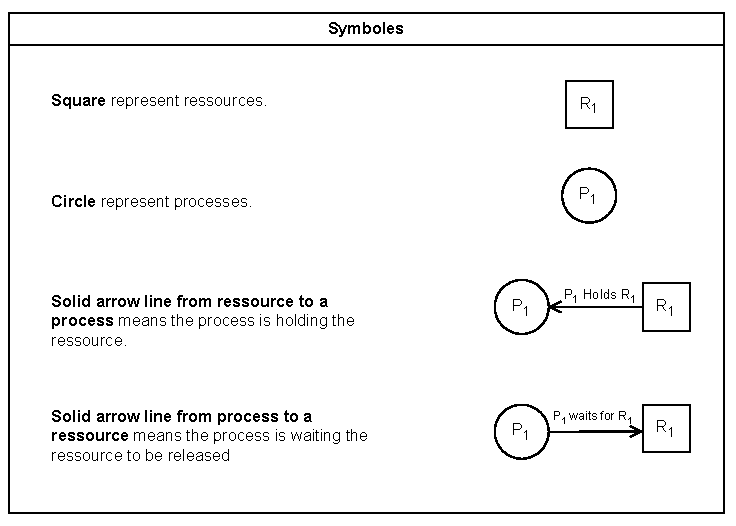
\includegraphics{Chapters/Diagram/Deadlock/sym.drawio.pdf}
\end{center}

\vspace{0.25cm}
\null
\section{Conditions for Deadlock}
\begin{prettyBox}{Coffman Conditions}{myblue}
Deadlock can arise if all the following conditions are met:
\begin{itemize}
    \item \textbf{Mutual Exclusion}: Only one process can hold a resource at a time.
    \item \textbf{Hold and Wait}: A process holding at least one resource is waiting for additional resources held by other processes.
    \item \textbf{No Preemption}: The \textbf{OS} cannot forcibly remove a resource from a process.
    \item \textbf{Circular Wait}: There is a cycle in the graph of two or more processes waiting for each other to release ressources.
\end{itemize}
\end{prettyBox}

\vspace{1cm}

\begin{center}
    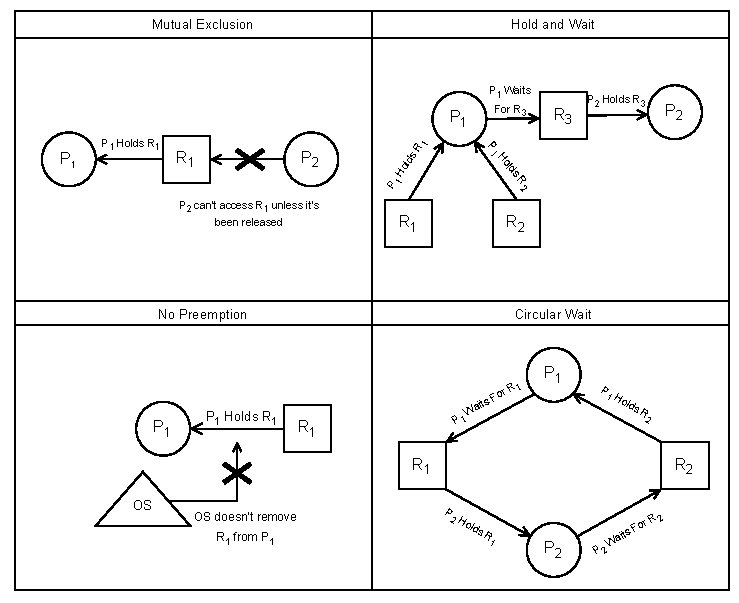
\includegraphics{Chapters/Diagram/Deadlock/coffman.drawio.pdf}
\end{center}

\newpage
\null
\section{Handling Deadlocks}
\begin{prettyBox}{Methods}{myblue}
\begin{itemize}
    \item \textbf{Ignore the Problem}: If resolving deadlocks is too costly, the \textbf{OS} may adopt a laissez-faire approach, ignoring deadlocks and requiring a system reboot if necessary.
    \item \textbf{Detection and Resolution}: The system detects deadlocks, often using algorithms like \textbf{DFS} on the resource allocation graph, and resolves them through one of the following strategies:
    \begin{itemize}
        \item \textbf{Preemption}: Reassign a resource from one process to another, which may lead to issues like inconsistency or lost progress.
        \item \textbf{Rollback}: Restore the system to a previously saved state and reallocate resources to avoid deadlock.
        \item \textbf{Termination}: Kill one or more processes involved in the deadlock to free resources.
    \end{itemize}
    
   \item \textbf{Avoidance}: Dynamically allocate resources in a way that avoids unsafe states, using the \textbf{Banker's Algorithm} to check the safety of each potential allocation before it is made.

    \item \textbf{Prevention}: Prevent deadlocks by ensuring at least one of Coffman’s conditions cannot occur:
    \begin{itemize}
        
\item \textbf{Mutual Exclusion}: Use serialized access (e.g., queues) to eliminate contention by ensuring resources are accessed in an orderly fashion. This doesn't remove mutual exclusion, but it allows the system to control priority, avoiding chaotic competition between processes.
        \item \textbf{Hold and Wait}: Require processes to request all the resources they need at the beginning. 
        While this prevents deadlocks, it can lead to inefficiency because resources may remain idle, and a resource may need to be released to be used by another.
        \item \textbf{No Preemption}: Allow preemption for certain resources by forcibly reallocating them. This
            approach is rarely practical due to the complexity of saving and restoring resource states.
        \item \textbf{Circular Wait}: Resources are assigned increasing numerical labels. Processes must request 
    resources in increasing order of their labels. If a process needs a previously allocated resource, it must first
    release any resources with higher labels before requesting the lower-numbered one. This ensures that no cycles can form in the resource allocation graph, preventing deadlock.
    \end{itemize}
\end{itemize}
\end{prettyBox}

 

\end{document}
